%%%%%%%%%%%%%%%%%%%%%%%%%%%%%%%%%%%%%%%%%%%%%%%%%%%%%%%%%%%%%%%%%%%%%%%%%%

% abnTeX2: Modelo de Trabalho Acadêmico em conformidade com
% as normas da ABNT

%%%%%%%%%%%%%%%%%%%%%%%%%%%%%%%%%%%%%%%%%%%%%%%%%%%%%%%%%%%%%%%%%%%%%%%%%%

\documentclass[english,
               brazil,
               bsc] %Opções bsc (TCC) e msc (Mestrado)
               {dcomp-abntex2}


%%%%%%%%%%%%%%%%%%%%%%%%%%%%%%%%%%%%%%%%%%%%%%%%%%%%%%%%%%%%%%%%%%%%%%%%%%
% Área para adição de pacotes extras
%%%%%%%%%%%%%%%%%%%%%%%%%%%%%%%%%%%%%%%%%%%%%%%%%%%%%%%%%%%%%%%%%%%%%%%%%%

% \usepackage{lipsum} %Retirar para a versão final do documento

%Utilize aqui seu pacote preferido para algoritmos
\usepackage[linesnumbered]{algorithm2e}

%%%%%%%%%%%%%%%%%%%%%%%%%%%%%%%%%%%%%%%%%%%%%%%%%%%%%%%%%%%%%%%%%%%%%%%%%%

%Compila o indice
\makeindex

\begin{document}

% Seleciona o idioma do documento (conforme pacotes do babel)
\selectlanguage{brazil}

% Retira espaço extra obsoleto entre as frases.
\frenchspacing

%%%%%%%%%%%%%%%%%%%%%%%%%%%%%%%%%%%%%%%%%%%%%%%%%%%%%%%%%%%%%%%%%%%%%%%%%%
% ELEMENTOS PRÉ-TEXTUAIS
%%%%%%%%%%%%%%%%%%%%%%%%%%%%%%%%%%%%%%%%%%%%%%%%%%%%%%%%%%%%%%%%%%%%%%%%%%

\pretextual

\titulo{AtalaIA: Compressão de modelos de detecção facial para dispositivos embarcados de baixo custo}
\autor{Luan Fabrício de Carvalho Lima Leite}
\orientador{Leonardo Nogueira Matos}
\coorientador{Rafael Andrade da Silva}
\curso{Ciência da Computação}

\inserirInformacoesPDF

\imprimircapa
\imprimirfolhaderosto*

\begin{dedicatoria}
   \vspace*{\fill}
   \centering
   \noindent
   \textit{Dedico este trabalho a minha família, amigos, professores e todos que de alguma forma me ajudaram a chegar até aqui.}
   \vspace*{\fill}
\end{dedicatoria}
% ---

% \begin{agradecimentos}


\end{agradecimentos}
% ---

% \begin{epigrafe}[]
    \vspace*{\fill}
	\begin{flushright}

		\textit{I may not have gone where I intended to go, \\
			but I think I have ended up where I needed to be. \\
			(Dougas Adams)}
	\end{flushright}
\end{epigrafe}
% ---

% resumo em português
\setlength{\absparsep}{18pt} % ajusta o espaçamento dos parágrafos do resumo
\begin{resumo}

Redes Neurais Convolucionais estão ficando cada vez mais populares para solução de diversos desafios, sendo um deles
o de reconhecimento facial, que é uma das tarefas onde essa abordagem já supera o ser humano.
Entretanto, esse método costuma exigir um alto poder de processamento e quantidade de memória, o que acaba
limitando o seu uso em casos de computação de borda com dispositivos embarcados.
Este trabalho tem como foco tratar esse problema, comprimindo um modelo de reconhecimento facial para que ele seja
embarcado e consiga realizar operações na borda, mantendo a acurácia alta e tempo de resposta baixo.
Para que esse objetivo seja cumprido, será necessário utilizar um modelo como base, para que ele seja comprimido e
avaliado, onde ele será escolhido a partir da comparação de soluções já existentes e utilizadas.
O modelo embarcado será avaliado com base em métricas como acurácia, F1 score, latência e ocupação de memória e
comparado a outras soluções existentes.

 \textbf{Palavras-chave}: CNN, Compressão de modelos, Visão computacional, Sistemas embarcados, Computação em borda,
 Reconhecimento facial
\end{resumo}

% resumo em inglês
\setlength{\absparsep}{18pt} % ajusta o espaçamento dos parágrafos do resumo
\begin{resumo}[Abstract]
 \begin{otherlanguage*}{english}
   Convolutional Neural Networks are becoming increasingly popular for solving various challenges, one of them being
   facial recognition, which is one of the tasks that this approach overcomes humans.
   However, this method usually requires a high computational power and amount of memory, which ends up limiting its
   use case in edge computing for embedded devices.
   This work focuses on addressing this issue, compressing a facial recognition model so that it is embedded and can
   perform operations at the edge, maintaining high accuracy and low response time.
   For this objective to be achieved, it will be necessary to use a model as a basis, so that it can be compressed and
   evaluated, where it will be chosen based on the comparison of the existing and used
   solutions.
   % TODO: traduzir essa parte
   To finish, this model will be embedded to perform operations on edge, both inference and processing on the device,
   from there, its effectiveness will be measured and compared with other solutions already created.

   \vspace{\onelineskip}

   \noindent
   \textbf{Keywords}: CNN. Model compression. Computer Vision. Embedded systems. Edge computing. Facial recognition.
 \end{otherlanguage*}
\end{resumo}



\mostrarlistadeILUSTRACOES
\mostrarlistadeQUADROS
\mostrarlistadeTABELAS
\mostrarlistadeCODIGOS
\mostrarlistadeALGORITMOS

% Lista de abreviaturas e siglas

\begin{siglas}
	\item[ABNT]{Associação Brasileira de Normas Técnicas}
	\item[abnTeX]{ABsurdas Normas para TeX}
  	\item[DCOMP]{Departamento de Computação}
	\item[UFS]{Universidade Federal de Sergipe}
	\item[ANN]{Rede Neural Artificial ou \textit{Artificial Neural network}}
	\item[CNN]{Rede Neural Convolucional ou \textit{Convolutional Neural Network}}
	\item[KB]{Kilobytes}
	\item[MB]{Megabytes}
	\item[API]{Interface de Programação de Aplicações ou \textit{Application Program Interface}}
	\item[IoT]{Internet das Coisas ou \textit{Internet of Things}}
\end{siglas}

% ---
% inserir lista de símbolos
% ---

\begin{simbolos}
  \item[$ \alpha $] Letra grega alfa
  \item[$ \Gamma $] Letra grega Gama
  \item[$ \Lambda $] Lambda
  \item[$ \zeta $] Letra grega minúscula zeta
  \item[$ \in $] Pertence
\end{simbolos}
% ---


\mostrarSUMARIO

%%%%%%%%%%%%%%%%%%%%%%%%%%%%%%%%%%%%%%%%%%%%%%%%%%%%%%%%%%%%%%%%%%%%%%%%%%
% ELEMENTOS TEXTUAIS
%%%%%%%%%%%%%%%%%%%%%%%%%%%%%%%%%%%%%%%%%%%%%%%%%%%%%%%%%%%%%%%%%%%%%%%%%%

\textual
\chapter{Introdução}

% TODO: Melhorar e aprofundar sobre ANN
Redes Neurais Artificiais, ou \textit{Artificial Neural Network} (ANN), são ferramentas poderosas para auxiliar a
sociedade.
Podendo ser utilizadas em diversas tarefas, como reconhecimento facial, onde a rede é treinada para realizar a
classificação da face da pessoa, permitindo que ela seja usada em várias áreas diferentes, indo de entretenimento até
segurança.

\section{Motivação}
% TODO: Talvez seja interessante rescrever para exaltar que o
% motivo foi o artigo
O uso de Redes Neurais Artificiais vem crescendo bastante no ramo de computação visual, principalmente desde 2012,
quando Redes Neurais Convolucionais ou \textit{Convolutional Neural Networks} (CNN) começaram a ser utilizadas para
classificação de imagens \cite{alexnet}.
Um dos usos desse tipo de rede é na detecção de face, que é muito relevante para a área de segurança e
vigilância, onde o modelo pode fazer a detecção do rosto de uma pessoa, abrir uma porta ou enviar uma notificação
para algum segurança.
Porém, essa abordagem necessita de uma quantidade elevada de poder computacional, tornando inviável que tal tipo de
produto seja embarcado e mantenha um baixo tempo de resposta, o que pode atrapalhar a experiência do usuário, ou
reduzir a efetividade da ação que será tomada.

Um dos principais problemas das Redes Neurais Profundas, como CNN, é que elas necessitam de um alto processamento e uso
de memória, o que acaba dificultando a sua execução em dispositivos com poder computacional e memória limitados (como os dispositivos embarcados).
Porém, existem técnicas que podem ser aplicadas para reduzir o poder computacional necessário, como o uso de
destilação de conhecimento \cite{hinton2015distilling}, poda e quantização.
Possibilitando a implantação do modelo em sistemas embarcados na borda, de forma que a latência do dispositivo seja
baixa.

\section{Objetivos}

O objetivo deste trabalho é comprimir uma Rede Neural Convolucional, permitindo que ela realize o reconhecimento
facial em microcontroladores, na borda.
Nele também serão tratadas formas de comprimir e otimizar o modelo, para que a sua versão final consiga ser embarcada
em um dispositivo com hardware limitado, mantendo acurácia alta e baixa latência.

\subsection{Objetivo específicos}
O trabalho estará completo se os seguintes objetivos forem alcançados:

\begin{itemize}
	% TODO: Reescrever, deixando claro que o objetivo é embarcar o modelo.
	% Deixar claro que é necessário que o modelo comprimido também tenha uma alta acurácia, F1-score etc.
	% Deixar claro que é necessário que o modelo comprimido não utilize poucos recursos computacionais
	%	(armazenamento, memória e uso de cpu) e que a latência também seja baixa.
	\item Aplicar técnicas de compressão e otimização em um modelo, assim reduzindo o uso de CPU e memória,
		o permitindo que seja embarcado.
	% TODO: Rever
	\item Validar performace do modelo, para garantir que a acurácia e F1-score do modelo seja mantida.
	\item Embarcar o modelo comprimido de forma que ele consiga realizar operações na borda, mantendo acurácia
		alta e baixa latência.
\end{itemize}

\section{Metodologia}
Para atingir o objetivo do estudo, foi necessário dividir o processo em algumas etapas, cada uma sendo
essencial para que o objetivo do trabalho fosse atingido. Sendo elas:

\begin{enumerate}
	\item \textbf{Levantamento do estado da arte:}

		Nessa etapa, são selecionados artigos que possuem o objetivo similar ao deste artigo,
		com base nesses artigos serão testadas novas técnicas para compressão de modelos.

	\item \textbf{Reprodução do estado da arte:}
		% TODO: Explicar melhor o que foi feito nesta etapa.
		% Verificar se ela irá aparecer na etapa final do trabalho.
		% TODO: Revisar

	\begin{enumerate}
		\item \textbf{Seleção de base e treino de modelos:}

			Nesta etapa, uma base de dados é selecionada e a partir dela serão desenvolvidos modelos,
			com o objetivo de atingir uma alta acurácia, sem sofrer \textit{overfitting}.

		\item \textbf{Aplicação de técnicas de compressão para Modelos:}

			Após definir e treinar os modelos, serão aplicadas técnicas de compressão, tendo como
			objetivo ter uma acurácia parecida com a do modelo original. Onde as técnicas aplicadas
			foram: poda, quantização e destilação de conhecimento.

		\item \textbf{Avaliação do desempenho:}

			Depois de treinar e aplicar técnicas de compressão, os dados dos modelos serão coletados e
			avaliados. Para realizar essa avaliação, será necessário utilizar um conjunto de testes.

		\item \textbf{Análise e comparação dos resultados:}

			Para finalizar, os dados dos modelos serão comparados e analisados. Com o objetivo de
			identificar o melhor modelo e descobrir quais foram os motivos para que esse modelo tenha se
			saído melhor, mesmo após a aplicação de compressão. Nesta etapa as métricas de acurácia e
			tamanho do modelo são avaliadas.
	\end{enumerate}

	\item \textbf{Escolha do modelo para reconhecimento facial:}

		Nesta etapa serão avaliados os modelos com base em métricas como acurácia, F1 score, latência e ocupação de
		memória. Após a avaliação será escolhido um modelo que servirá como base nas próximas etapas.

	\item \textbf{Compressão e implantação do modelo em hardware limitado:}

		Depois de escolher um modelo de reconhecimento facial, ele será comprimido de forma que possa ser executado
		em sistemas embarcados, mantendo a acurácia alta e latência baixa.

	\item \textbf{Desenvolvimento do estudo de caso:}

		Com o modelo final comprimido ao ponto de ser implantado em um sistema embarcado, será desenvolvida uma aplicação 	 	 que servirá como experimento para avaliar a eficácia do modelo dentro de dispositivos com hardware limitado.

\end{enumerate}

As etapas 3, 4 e 5 serão realizadas no Trabalho de Conclusão de Curso 2.

\section{Estrutura do documento}
Este documento foi dividido em capítulos, onde cada um apresenta uma proposta diferente:
\begin{itemize}
	\item Capítulo 2 - \textbf{Conceitos Básicos}: Apresenta os tópicos principais para o entendimento
		do trabalho.
	\item Capítulo 3 - \textbf{Trabalhos Relacionados}: Apresenta uma revisão dos trabalhos
		relacionados ao tema do trabalho.
	\item Capítulo 4 - \textbf{Resultados Preliminares}: Apresenta os resultados preliminares dos
		experimentos realizados durante o trabalho.
	\item Capítulo 5 - \textbf{Planos de continuidade}: Contém o planejamento da continuidade do
		Trabalho de Conclusão 2.
\end{itemize}

\chapter{Conceitos básicos}\label{cap_conceitos}

\chapterprecis{Isto é uma sinopse de capítulo. A ABNT não traz nenhuma
normatização a respeito desse tipo de resumo, que é mais comum em romances
e livros técnicos.}\index{sinopse de capítulo}

\section{Redes Neurais Artificiais}\label{cap_conceitos_ann}
% ---
Redes Neurais Artificiais (ANNs), são neurônios interconectados que realizam um processamento simples. Dentro dessa
estrutura cada neurônio reforça ou enfraquece a conexão com um dos neurônio da coluna anterior, assim replicando
o processo de aprendizagem do cérebro humano. A \autoref{cap_conceitos_ann_exemplo_ann} exemplifica uma ANN bem
simples.

\begin{figure}[htb]
	\caption {\label{cap_conceitos_ann_exemplo_ann}Exemplo de uma ANN}
	\begin{center}
		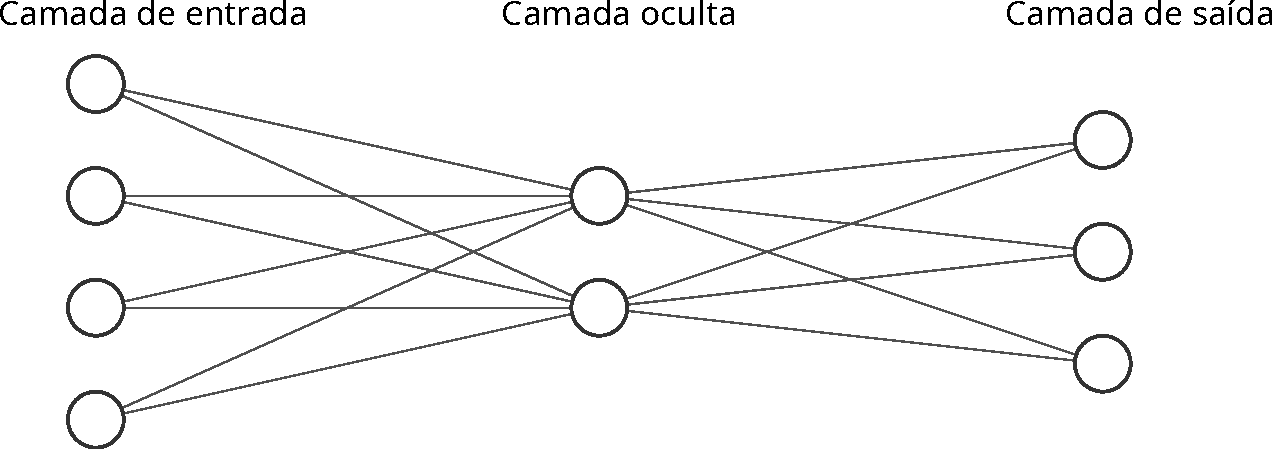
\includegraphics[scale=0.5]{Imagens/exemplo_nn}
	\end{center}
	\legend {Fonte: Autor}
\end{figure}

O neurônio é uma parte fundamental de uma ANN, nele que o aprendizado é armazenado através do reforço de conexões com
outros neurônio. Esse reforço é o peso da conexão, ele é multiplicado pela entrada e somado com os outros valores,
como é demonstrado na equação \ref{eq_neuronio} (onde $x$ é um vetor com os valores de entrada do neurônio e $w$
é um vetor com os pesos de cada entrada). Depois disso os valores passam por uma função de ativação $g(x)$ (\ref
{eq_ativacao}), que é responsável por "tratar" esses dados de saída antes que eles sejam passados para próxima etapa.

\begin{equation}\label{eq_neuronio}
u = \sum x_i w_i
\end{equation}
\begin{equation}\label{eq_ativacao}
y = g(u + b)
\end{equation}

\begin{figure}[htb]
	\caption {\label{cap_conceitos_ex_neuronio} Exemplo de um neurônio artificial}
	\begin{center}
		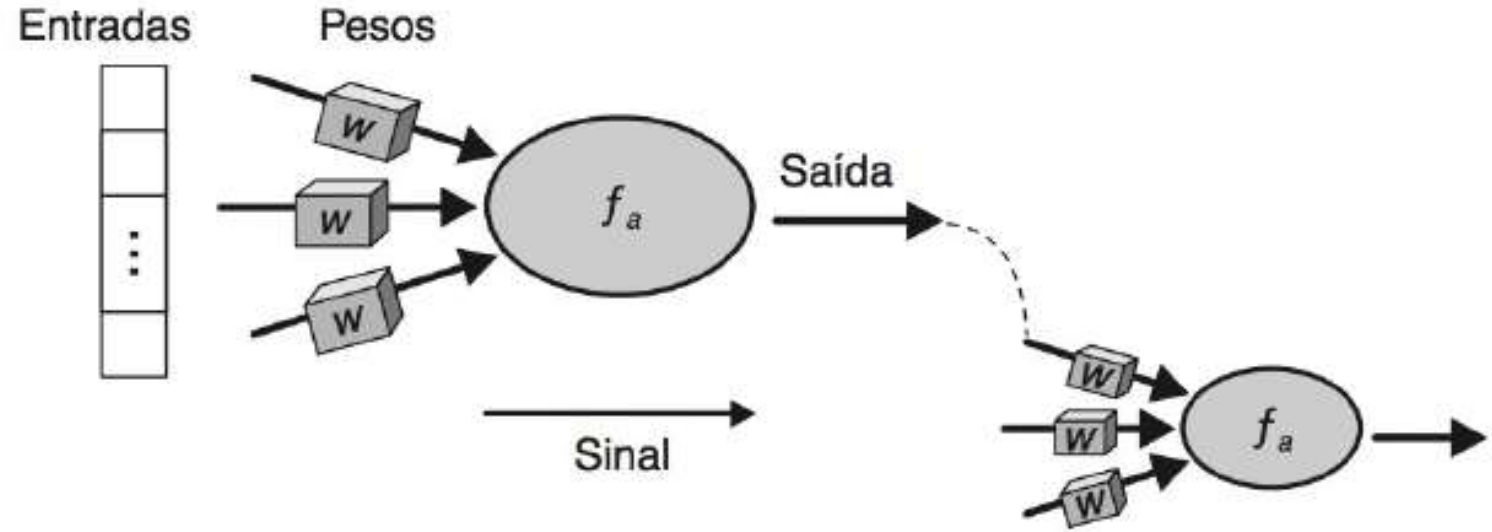
\includegraphics[scale=0.3]{Imagens/exemplo_neuronio_artificial}
	\end{center}
	\legend{Fonte: \cite{ml-faceli}}
\end{figure}

\section{Redes Neurais Convolucionais}\label{cap_conceitos_cnn}
% ---
Redes Neurais Convolucionais (CNNs) são Redes Neurais Artificiais (ANN)
que utilizam a operação de convolução para o processamento e análise de dados no formato de \textit{grid}(grade).
Por exemplo, uma série temporal que pode ser representada no formato de \textit{grid} 1-D,
ou uma imagem, que pode ser representada no formato 2-D. \cite{Goodfellow-et-al-2016}
Onde, LeNet \cite{lenet}, Residual Network (ResNet) \cite{resnet} e AlexNet \cite{alexnet} são alguns exemplos de CNNs
famosas.
% (TODO: Adicionar exemplos)

A arquitetura de uma CNN é composta por camadas convolucionais (\ref{cap_conceitos_cnn_conv}),
\textit{pooling} (\ref{cap_conceitos_cnn_pooling}) e totalmente conectadas (\ref{cap_conceitos_cnn_totalmente}),
como podemos ver na \autoref{exemplo_lenet}.

\begin{figure}[htb]
	\caption {\label{exemplo_lenet} Arquitetura da LeNet}
	\begin{center}
		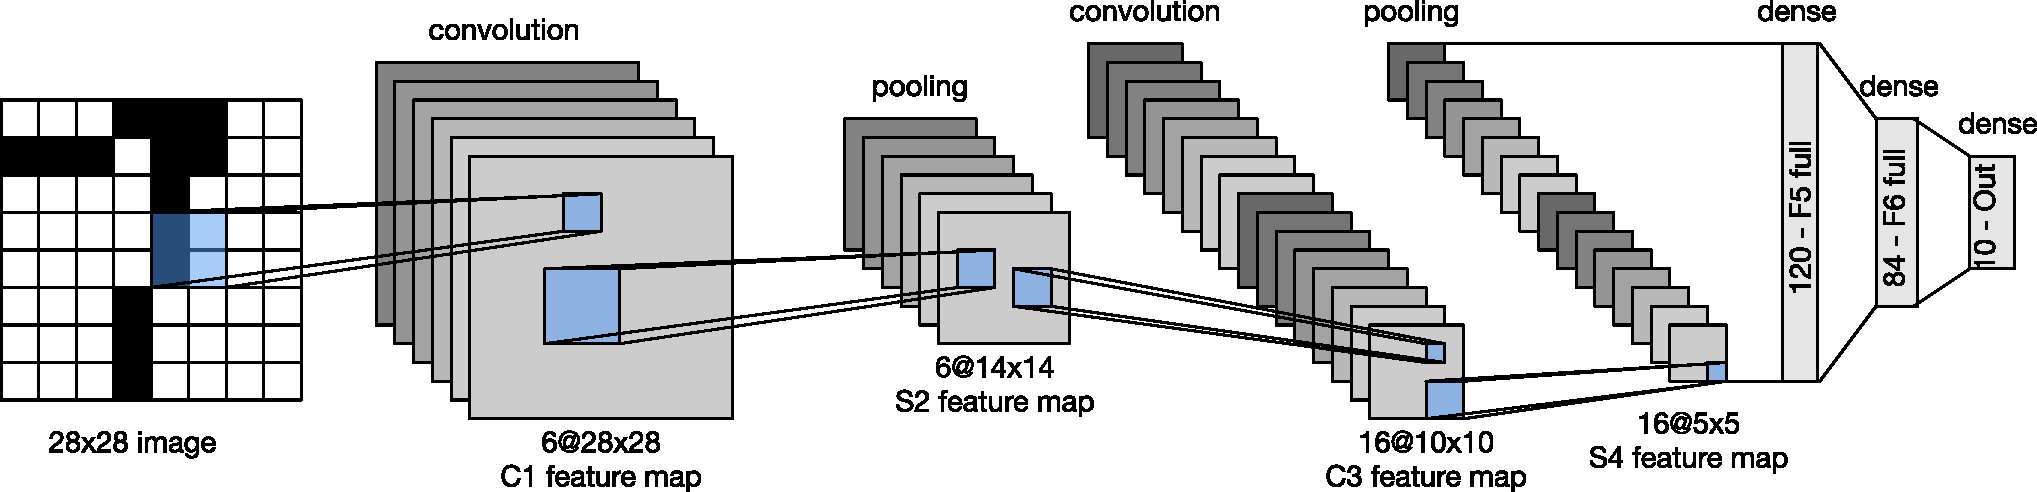
\includegraphics[scale=0.5]{Imagens/lenet}
	\end{center}
	\legend{Fonte: \cite{zhang2023dive}}
\end{figure}

\subsection{Camada de Convolução}\label{cap_conceitos_cnn_conv}
Nessa camada são aplicados filtros (matriz de pesos) nos dados de entrada,
onde esses filtros deslizam cada célula da imagem executando operações de multiplicação e soma
em cada elemento da matriz de entrada, com o objetivo de gerar um mapa de características (\textit{feature map}).
O objetivo desses filtros é realçar as características dos dados de entrada, como curvas, linhas e outros padrões.
% (TODO: Adicionar figuras, referências e detalhar mais)

\subsection{Camada de \textit{pooling}}\label{cap_conceitos_cnn_pooling}
% ---
A abordagem da camada de \textit{pooling} é um pouco parecida com a camada de convolução,
uma matriz desliza pelas células da imagem, salvando apenas o maior valor dessa área na matriz de saída.
A partir disso, a camada consegue reduzir o tamanho da matriz de entrada, fazendo com que o poder computacional
necessário seja reduzido, junto com o uso de memória.
(TODO: Adicionar figuras, referências e detalhar mais)

\subsection{Camada totalmente conectada}\label{cap_conceitos_cnn_totalmente}
% ---
A camada totalmente conectada (\textit{fully connected layer}) é a camada final de uma CNN.
Depois das camadas anteriores extraírem as características da imagem, a camada totalmente
conectada as interpreta e gerar uma resposta.
(TODO: Revisar texto)

\section{\textit{Data augmentation}}
% ---
CNNs tem um ótimo desempenho em tarefas de visão computacional. Entretanto esse tipo de rede neural precisa de uma
grande quantidade dados para não sofrer de \textit{overfitting} (superajuste). \cite{shorten2019survey}
Esse é o objetivo do \textit{data augmentation} (aumento de dados), gerar mais dados a partir de um conjunto de dados
que já existe, aplicando algumas transformações geométricas ou espaciais, ou realizam injeção de ruído nas imagens
originais.

% TODO: Adicionar exemplo de data augmentation.

\section{Transferência de conhecimento}\label{conceitos_transferencia}
% ---
Transferência de conhecimento consiste em usar um modelo pré-treinado em uma base de dados específica e aproveitar
o conhecimento adquirido durante esse treinamento para um novo conjunto de dados.
É necessário que o problema do \textit{dataset} (conjunto de dados) atual seja um subconjunto do \textit{dataset}
que foi usado para treinar o modelo base.

Para realizar a transferência de conhecimento é necessário adaptar a camada de entrada e de saída
(totalmente conectada) do modelo base, para que ocorra um pré-processamento dos dados de entrada
(antes deles serem passados para o modelo base), além disso é necessário definir e treinar a camada totalmente
conectada com o \textit{dataset} do problema.

\section{Métodos de compressão para Redes Neurais}
ANNs são utilizadas em várias aplicações, demonstrando habilidades extraordinárias no campo de visão computacional.
No entanto, redes com arquiteturas complexas são um desafio para a implantação em tempo real e necessitam de uma
grande quantidade de energia e poder computacional \cite{LIANG2021370}.
Por causa disso foram desenvolvidos métodos para reduzir o tamanho dessas redes, as tornando mais eficiente.
Nesse trabalho os métodos de poda (\ref{poda}), quantização (\ref{quantizacao}) e destilamento do conhecimento
(\ref{conceitos_destilamento}) serão usados.

\subsection{\textit{Pruning}(Poda)}\label{poda}
A poda de redes neurais tem como objetivo principal remover pesos ou neurônios que são
redundantes ou irrelevantes para o problema, além disso reduz o \textit{overfitting}(superajuste).
(TODO: escrever sobre poda de redes neurais)

% Redes neurais costumam usar muito recurso computacional e otimizar o uso dos recursos é muito importante para
% aplicações de grande escala. A poda de redes neurais tem como objetivo principal remover pesos ou neurônios que são
% redundantes ou irrelevantes para o problema, além disso reduz o \textit{overfitting}(superajuste).

\subsection{Quantização}\label{quantizacao}

% Quantization reduces computations by reducing the precision of the datatype. Weights, biases, and activations
% may be quantized typically to 8-bit integers although lower bit width implementations are also discussed including
% binary neural networks. Both pruning and quantization can be used independently or combined.

Quantização reduz a computação diminuindo a precisão dos tipos de dados. Pesos, \textit{bias} (vieses) e ativações
geralmente devem ser quantizadas para inteiros de 8 bit, embora implementações menores que 8 bit sejam discutidas
incluindo redes neurais binárias. \cite{LIANG2021370}

% (TODO: Escrever sobre quantização)

\subsection{Destilamento de conhecimento (Professor-Aluno)}\label{conceitos_destilamento}

Destilamento de conhecimento ou \textit{knowledge distillation} \cite{hinton2015distilling}, é uma técnica que tem
como objetivo treinar um modelo Aluno (menor e sem pré-treinamento) com um modelo Professor
(maior e com pré-treinamento). Ela é amplamente utilizada para as áreas de visão computacional e linguagem natural,
e tem como objetivo reduzir o tamanho do modelo final (Aluno).

Para transferir o conhecimento do modelo Professor para o Aluno, a técnica utiliza os \textit{logits} (entrada da
função de ativação final \textit{softmax}) no lugar da classe prevista. Além disso, são utilizado os
\textit{soft targets} (probabilidades das classes previstas pelo modelo Professor) junto com os
\textit{hard targets} (classe esperada). Então, o Aluno é treinado com uma porcentagem $\alpha$ do erro com o
\textit{hard target} e $\alpha - 1$ do erro com \textit{soft target}, assim é calculado o erro do aluno.

% NOTE: Talvez detalhar a temperatura?

% Destilamento de conhecimento ou \textit{knowledge distillation} \cite{hinton2015distilling}, é uma técnica de
% treinamento que utiliza dois modelos, Professor que é um modelo mais robusto e pré-treinado para o problema, e
% o modelo Aluno que é o modelo que (geralmente) é mais leve que o professor e não possui nenhum pré-treinamento.
% Para destilar o conhecimento do professor para o estudante, utilizamos os \textit{logits}, que são os valores de
% entrada da camada \textit{softmax}, então os \textit{logits} do \emph{professor} são comparados com os do
% \emph{estudante}.
% TODO: escrever sobre destilamento de conhecimento

\section{Otimização Bayesiana}
% ---


% TODO: Escrever sobre otimização Bayesiana.

\chapter{Trabalhos relacionados}\label{cap_trabalhos_relacionados}

Neste capítulo serão discutidos os trabalhos relacionados à compressão de CNN com foco em dispositivos
embarcados.

\section{Trabalhos acadêmicos}

Os seguintes critérios de busca foram utilizados para filtrar os trabalhos acadêmicos:

\begin{itemize}
	% TODO: Olhar
	\item Portal de periódicos utilizada foi a CAPES CAFE.
	\item A string de busca foi a seguinte: "face recognition" and "esp32".
	\item O seguintes filtros foram utilizados:
	\begin{itemize}
		\item Idioma: Inglês.
		\item Revisado por pares: Sim.
	\end{itemize}
---
	\item Os artigos devem ser relacionado ao tema de CNN com compressão para sistemas embarcados.
	\item Trabalhos publicados entre 2020 e 2023.
	\item Trabalhos escritos em inglês.

	As bases utilizadas foram: IEE Eletronic Library, ACM Digital Library e Science Citation Index Expanded.
	Utilizando a seguinte string de busca:
	\item "CNN"  AND "EMBEDDED" AND "Edge devices" AND ("Pruning" OR "Knowledge distillation" OR "Quantization")
\end{itemize}

\subsection{\textit{A Resource Constrained Pipeline Approach to Embed Convolutional Neural Models (CNN)}}
O objetivo deste trabalho de dissertação \cite{rafael} é elaborar um modelo de detecção de placas de trânsito que seja
computacionalmente e energeticamente barato. Para atingir esse objetivo, foi elaborada uma pipeline de compressão,
começando pela destilação de conhecimento, e partindo para poda e quantização.

O resultado alcançado foi uma CNN capaz de detectar placas de trânsito, consumindo 59KB de espaço, com $85,91\%$ de
acurácia e F1-Score igual a $85,80\%$, atingindo um tempo de inferência de 80 ms no ESP32 e 83 ms no ESP32-2.

\subsection{\textit{IMPROVED FACE DETECTION ACCURACY USING HAAR CASCADE CLASSIFIER METHOD AND ESP32-CAM FOR IOT-BASED HOME DOOR SECURITY}}

\subsection{\textit{Intelligent security system based on face recognition and IoT}}
Este trabalho tem como objetivo desenvolver um protótipo de sistema de segurança baseado em reconhecimento facial,
utilizando \textit{Internet of Things} (IOT). Para atingir esse objetivo, os autores utilizam um ESP32-CAM como componente
principal para realizar a coleta e reconhecimento da face.

% TODO:Melhorar
O resultado alcançado foi um protótipo que é capaz de verificar se a face capturada é conhecida, caso seja, ela acende um
LED verde, caso contrário um LER vermelho é ligado. Além disso, foi levantada uma lista de pontos fortes, fracos, ameaças
e oportunidade do protótipo.

% TODO:Melhorar (usar artigo como base)
\begin{center}
\begin{table}[htb]
\centering
\ABNTEXfontereduzida
\caption[]{}
\label{tabela_swot}
\begin{tabular}{ |c|c| }
	\hline
	Eficiência energética \\
	Custo x benefício \\
	\hline
\end{tabular}
\legend{}
\end{table}
\end{center}

\chapter{Experimentos e resultados}\label{experimentos}

Neste capítulo serão apresentados os experimentos feitos durante o TCC. Eles tiveram como
finalidade avaliar o uso de métodos e técnica de compressão de modelos, focado em dispositivos
embarcados. Nele serão apresentados o dispositivo utilizado (\autoref{sec_dispositivo}),
modelos usados (\autoref{sec_modelo_utilizado}), métodos de treinamento (\autoref{sec_treinamento_modelo}),
o método de avaliação do modelo (\autoref{sec_avaliacao_modelo}), \textit{datasets} utilizados
(\autoref{sec_datasets}) e resultados (\autoref{sec_resultados}).

\section{Dispositivos utilizados}\label{sec_dispositivo}
% Para avaliar os modelos, foram usados diversos dispositivos para que seja possível medir a sua performance em mais de um
% ambiente.
%
% \subsection{Desktop}\label{sec_dispositivo_desktop}
% Para auxiliar na etapa de avaliação dos modelos, foi utilizado um computador com o processo AMD Ryzen 5 4600G e 16GB de
% memória ram, ele serviu como base para avaliação por ser um dispositivo com grande poder computacional.
%
% Além disso, ele foi o ambiente de desenvolvimento do projeto, onde foram desenvolvidos os benchmarks e utilitários
% usados no trabalho.
%
% \subsection{ESP32-S3}\label{sec_dispositivo_esp}
O ESP32-S3 N16R8 foi escolhido pelo seu custo-benefício, sendo um aparelho poderoso considerando o seu baixo
custo e consumo energético. Além disso, esse dispositivo possui 16 MB de memória flash e 8 MB de PSRAM,
permitindo que modelos maiores sejam portados para esse dispositivo sem redução de parâmetros, podendo afetar o
tempo de inferência do modelo.

Para executar os modelos no ESP foi utilizado o projeto person-detection do repositório esp-tflite-micro da Espressif
\footnote{Disponível em: \url{https://github.com/espressif/esp-tflite-micro/tree/master} Acessado em Março de 2025}.
A partir desse projeto, os modelos foram portados, sendo necessário realizar algumas alterações no projeto,
para suportar o tamanho dos modelos e suas camadas, e adicionar alguns utilitários, como um \textit{log} com
o uso da memória.

\section{Modelos utilizados}\label{sec_modelo_utilizado}
Para realizar os experimentos, os modelos \textbf{MobileFaceNet}, \textbf{Rafael-2} e \textbf{MobileNetV3Small}
foram utilizados como teste, tanto na etapa de treinamento (\autoref{sec_treinamento_modelo}) quanto de avaliação
(\autoref{sec_avaliacao_modelo}).

Para treinar os modelos, foi utilizada a plataforma kaggle\footnote{
Disponível em: \url{https://www.kaggle.com/}. Acessado em Março de 2025}, o \textit{dataset} utilizado foi
\textit{Labeled Faces in the Wild} (LFW) \footnote{
Disponível em: \url{https://www.kaggle.com/datasets/luhtookyaw/lfwpreparedtriplets}. Acessado em Março de 2025.},
onde os métodos de treinamento \textit{Triplet Loss} e \textit{Triplet Distillation}
\cite{triplet_distillation_face_recognition} foram utilizados, pois são eficazes para melhorar a precisão do modelo,
no contexto de reconhecimento facial.
Além disso os modelos foram treinados considerando com imagens R8G8B8, cada imagem tem seus pixels representados por
triplas de 8 bits, contendo o valor das cores vermelho, verde e azul, respectivamente.

% TODO: Ver se eu posso deixar esse footnote
Para validar os resultados de cada modelo, foi criado o repositório model-eval\footnote{
Disponível em: \url{https://github.com/LuanFabricio/model-eval}. Acessado em Março 2025.}, para ser utilizado junto com o
\textit{dataset} Faces - UFS \cite{leandro}.
Onde o método de validação consiste em comparar uma imagem com \textit{flip} com todo o \textit{dataset}, e definindo
a classe prevista pelo modelo aquela que possui menor distância de cosseno.
% \subsection{MobileFaceNet}
% O modelo utilizado foi o MobileFaceNet, pois ele mantém uma acurácia acima de 90\% na tarefa de detecção de faces,
% com tempo de inferência e baixa pegada de memória \cite{leandro}.

MobileFaceNet é um modelo focado para fazer reconhecimento de faces em tempo real em dispositivos móveis,
assim possuindo uma baixa pegada de memória, abaixo de 5MB e mantendo uma acurácia alta, acima de 90\% \cite{leandro}.

% \subsection{Rafael-2}
Rafael-2 é uma variação do modelo Rafael \cite{rafael}, adaptada para realizar a tarefa de reconhecimento facial.
Como o modelo base é simples e focado para dispositivos embarcados, ele possuí uma baixa quantidade de parâmetros,
 o que melhora a performance do modelo em dispositivos embarcados.

% \subsection{MobileNetV3Small}
MobileNetV3Small é uma variação do MobileNetV3, com uma quantidade reduzida de parâmetros, reduzindo a sua pegada de
memória e aumentando a performance.
% TODO: CITAR ARTIGOS

% ADICIONAR TABELA COM O CONSUMO DE RECURSOS DO MODELO
% \begin{table}[htb]
% \centering
% \ABNTEXfontereduzida
% \caption[Recurso utilizado por modelo]{Recurso ocupado pelos modelos utilizados}
% \label{tabela_acuracia_1}
% \begin{tabular}{ |c|c|c|c|c| }
% 	\hline
% 	\textbf{Modelo} & \textbf{Quantização} & \textbf{Tamanho do arquivo (TFLite)} \\
% 	\hline
% 	MobileFaceNet 		& - 	& 4.5MB \\
% 	MobileFaceNet 		& uint8 & 1.5MB \\
% 	Rafael-2 		& - 	& 1.4MB \\
% 	Rafael-2 		& uint8 & 356KB \\
% 	MobileNetV3Small 	& - 	& 1.4MB \\
% 	\hline
% \end{tabular}
% \legend{Fonte: Autor}
% \end{table}

\section{Método de treinamento do modelo}\label{sec_treinamento_modelo}
Para fazer o treinamento dos modelos, foi necessário utilizar a técnica de \textit{Triplet Distillation}
\cite{triplet_distillation_face_recognition},
para que seja possível medir o quão próximo as \textit{embeddings} de uma imagem são parecidas com as de outra.
Essa técnica usa três imagens: \textbf{âncora}, que é serve como imagem base; \textbf{positiva},
que é uma variação da mesma categoria da \textbf{âncora}; e a \textbf{negativa}, que pertence a outra categoria.

No contexto de reconhecimento facial, os \textit{embeddings} das imagens \textbf{âncora} e \textbf{positivas}
devem possuir uma distância de cosseno pequena, enquanto o vetor de característica das imagens
\textbf{âncoras} e \textbf{negativas} devem possuir uma distância de cosseno alta.

\subsection{\textit{Triplet Loss}}
Para realizar o treinamento do modelo MobileFaceNet, foi utilizada a técnica \textit{triplet loss}
\cite{triplet_distillation_face_recognition}. Ela tem como objetivo comparar os \textit{embeddings} de três imagens,
utilizando a distância de cosseno ($D$) de um embedding ($x_i^j$) comparado com outro ($x_i^k$).
%Essa técnica utiliza é descrita pela fórmula \ref{eq_triplet_loss}

\begin{equation}\label{eq_triplet_loss}
	Loss = \frac 1 N \sum _i ^N max(D(x_i^a, x_i^p) - D(x_i^a, x_i^n) + m, 0))
\end{equation}
%
% \begin{equation}\label{eq_triplet_loss_teacher_dist}
% 	d = max(T(x_i^a, x_i^n) - T(x_i^a, x_i^p), 0)
% \end{equation}
%

Na equação \ref{eq_triplet_loss}, é a função \textit{Loss} utilizada para treinar o modelo. Onde, $x_i^a$ é
a imagem âncora, $x_i^p$ é a imagem positiva e $x_i^n$ é a imagem negativa, todas referentes a i-ésima
tripla e $m$ é um hiperparâmetro que define a margem entre o par positivo e par negativo.
Então, quanto mais parecidos forem os \textit{embeddings} da imagem âncora com a imagem positiva,
menor será a perda, sendo o inverso para a âncora com a imagem negativa.

\subsection{\textit{Triplet Distillation}}
Para realizar o treinamento dos modelos MobileNetV3 e Rafael-2, foi utilizada a técnica de
\textit{Knowledge Distillation} \cite{hinton2015distilling} com \textit{Triplet Loss}, conhecida como
\textit{triplet loss} \cite{triplet_distillation_face_recognition}.
Ela utiliza cálculo da \textit{Loss Function} (\ref{eq_triplet_loss}) como base, adicionando a distância entre os
\textit{embeddings} do modelo estudante e do modelo professor, como pode ser visto na fórmula
\ref{eq_triplet_distillation}.

\begin{equation}\label{eq_triplet_distillation}
	Loss = \frac 1 N \sum _i ^N max(D(x_i^a, x_i^p) - D(x_i^a, x_i^n) + d, 0))
\end{equation}

\begin{equation}\label{eq_triplet_loss_teacher_dist}
	d = max(T(x_i^a, x_i^n) - T(x_i^a, x_i^p), 0)
\end{equation}

Onde $T$ (\ref{eq_triplet_loss_teacher_dist}) é a distância entre os \textit{embeddings} do modelo estudante e
professor, e $d$ (\ref{eq_triplet_distillation}) é utilizado como uma margem dinâmica entre par positivo e negativo.

% TODO:
% - Citar modelos treinados (Triplet Distillation)
% 	- Rafael
% 	- MobileNetV3Small

\section{Método de avaliação}\label{sec_avaliacao_modelo}
Para avaliar o modelo, primeiro, as características de cada imagem e sua versão espelhada
(\textit{flip} horizontal) são extraídas pelo modelo. Depois é realizada a verificação da face,
calculando a distância de cosseno entre os vetores de características
\cite{triplet_distillation_face_recognition}, onde a imagem com menor distância é considerada a previsão do
modelo. A \autoref{exemplo_flip_lfw} é um exemplo da imagem original e sua versão com \textit{flip}.

\begin{figure}[htb]
	\begin{center}
		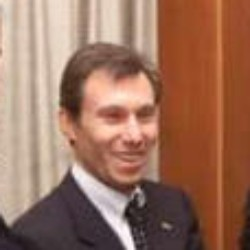
\includegraphics[scale=0.5]{Imagens/exemplo_flip_01}
		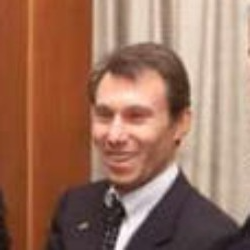
\includegraphics[scale=0.5]{Imagens/exemplo_flip_02}
	\end{center}
	\caption {\label{exemplo_flip_lfw}Exemplo de uma imagem e sua versão com \textit{flip}}
	\legend {Fonte: LFW} %Colocar fonte do LFW
\end{figure}
% TODO: DETALHAR

% Para gerar as estatísticas de modelo, foi calculada a precisão e acurácia de cada um, junto com o seu tempo de
% inferência. Onde

\section{\textit{Datasets}}\label{sec_datasets}
Nessa seção serão apresentados os dois \textit{datasets} utilizados, \textit{Labeled Faces in the Wild} (LFW),
que foi utilizado para o treinamento dos modelos, e Faces - UFS, que foi utilizado para a validação dos modelos.

\subsection{\textit{Labeled Faces in the Wild}}
Este \textit{dataset} possui imagens da face de várias celebridades, classificadas com o nome da pessoa.
Para esse trabalho, foi utilizada uma variação do LFW, que agrupa as imagens em triplas, \textbf{âncora},
\textbf{positiva} e \textbf{negativa}, para ser utilizado como dataset de treinamento, seguindo a técnica
de \textit{triplet distillation} \cite{triplet_distillation_face_recognition}.


Para realizar o treinamento do modelo, foi utilizada uma variação do \textit{dataset}
\textit{Labeled faces in the Wild} (LFW), que possui várias amostras contendo triplas com as imagens das faces,
assim facilitando o uso da técnica de \textit{triplet distillation} para o treinamento.

\subsection{Faces - UFS}\label{subsec_dataset_faces_ufs}
Este \textit{dataset} possui faces coletadas de alunos da Universidade Federal de Sergipe (UFS) \cite{leandro}.
Para coletar essas imagens, foi disponibilizado um estande com uma câmera, monitor, teclado e mouse, permitindo
que qualquer pessoa pudesse salvar uma imagem com o seu nome.

Esse \textit{dataset} foi utilizado na etapa de validação do modelo (\ref{sec_avaliacao_modelo}), por apresentar faces
novas e com um padrão diferente do LFW, já que o seu público consiste em celebridades, principalmente dos Estados
Unidos. Enquanto o \textit{dataset} coletado na UFS possui um público diferente, estudantes ou funcionários da UFS.

\section{Resultados}\label{sec_resultados}
Para obter os resultados, primeiro foram definidas as métricas que serão usadas para avaliar os modelos. Em seguida,
cada modelo foi submetido ao método de avaliação escolhido (\autoref{sec_avaliacao_modelo}), com o objetivo de
validar e comparar o desempenho na tarefa de reconhecimento facial de cada um, junto com o seu tempo de execução.

Para realizar a avaliação na tarefa de reconhecimento facial, os modelos foram executados em um computador com um
AMD Ryzen 5 4600G e em um Raspberry Model B. Na etapa de avaliação de performance em microcontroladores, foi utilizado
o ESP32-S3 N16R8, descrito na \autoref{sec_dispositivo}.

\subsection{Métricas usadas}\label{sect_restultados_metricas}
Para avaliar o desempenho, foram utilizadas as métricas de precisão (\ref{sect_restultados_metricas_precisao})
e acurácia (\ref{sect_restultados_metricas_acuracia}). Como a avaliação é binária, a imagem prevista é a imagem
verdadeira, também foi utilizada a matriz de confusão, para facilitar o entendimento dos acertos e erros, quanto
facilitar o cálculo da precisão e acurácia.

\label{sect_restultados_metricas_precisao}
A precisão pode ser calculada pela \autoref{eq_precisao} e a acurácia pela \autoref{eq_acuracia}.
Onde a variável $TP$ indica o valor que foi previsto corretamente como verdadeiro, enquanto a variável $FP$ indica o
valor que foi previsto falsamente como verdadeiro.
Considerando o método de avaliação utilizada, a variável $TP$ indica os casos onde o modelo escolheu corretamente a
imagem, e a variável $FP$  indica quando o modelo escolheu a imagem errada.

\begin{equation}\label{eq_precisao}
	\text{Precisão} = \frac {TP} {TP + FP}
\end{equation}

\label{sect_restultados_metricas_acuracia}
\begin{equation}\label{eq_acuracia}
	\text{Acurácia} = \frac {TP + TN} {TP + TN + FP + FN}
\end{equation}

\subsection{Avaliação do modelo}
Para a avaliação do modelo, o método descrito na \autoref{sec_avaliacao_modelo} foi executado 10 vezes,
utilizando o \textit{dataset} Faces - UFS (\ref{subsec_dataset_faces_ufs}), medindo o tempo médio de inferência,
desvio padrão e acurácia de cada execução.
Com isso, esses resultados, foi gerada a \autoref{acuracia_tempo_inferencia_modelos_desktop}, onde as
métricas são dos modelos descritos na \autoref{sec_modelo_utilizado}.


\begin{table}[htb]
\centering
\ABNTEXfontereduzida
\caption[Acurácia e tempo de inferência com o dataset Faces - UFS (Desktop)]{Acurácia e tempo de inferência com o dataset Faces - UFS (Desktop)}
\label{acuracia_tempo_inferencia_modelos_desktop}
\begin{tabular}{ |c|c|c|c|c| }
	\hline
	\textbf{Modelo} & \textbf{Quantização} & \textbf{Acurácia (\%)} & \textbf{Tempo médio de inferência (ms)} & \textbf{Método de treinamento} \\
	\hline
	MobileFaceNet 	&-	& 	100.00  & $129 \pm 2.002$ & Pré-treinado + \textit{Triplet Loss} \\
	MobileFaceNet 	&uint8	& 	100.00  & $443 \pm 2.734$ & Pré-treinado + \textit{Triplet Loss} \\
	Rafael-2	&-	& 	 3.25 & $115 \pm 0.553$ & \textit{Triplet Distillation} \\
	Rafael-2	&uint8	& 	 24.03& $103 \pm 0.209$ & \textit{Triplet Distillation} \\
	MobileNetV3Small&-	& 	 7.14& $37 \pm 0.701$ & \textit{Triplet Distillation} \\
	\hline
\end{tabular}
\legend{Fonte: Autor}
\end{table}

A \autoref{acuracia_tempo_inferencia_modelos_desktop} contém os resultados dos testes feitos com os modelos
MobileFaceNet, Rafael-2 e MobileNetV3Small, mostrando o tipo de quantização que foi feito, acurácia, tempo
médio de inferência e o método de treinamento.

Com isso, é possível notar que o modelo que o melhor modelo foi o MobileFaceNet, por conta da sua estrutura
mais robusta que tem o foco na tarefa de reconhecimento facial. Além disso, fica evidente a diferença entre
o tempo de inferência do MobileFaceNet quantizado e não quantizado, isso se deve pelo ambiente de execução
do TensorFlowLite, que em tempo de execução converte os pesos quantizados de inteiro de 8 bits para float.


\begin{table}[htb]
\centering
\ABNTEXfontereduzida
\caption[Acurácia e tempo de inferência com o dataset Faces - UFS (Raspberry Pi Model B)]{Acurácia e tempo de inferência com o dataset Faces - UFS (Raspberry Pi Model B)}
\label{acuracia_tempo_inferencia_modelos_raspberry}
\begin{tabular}{ |c|c|c|c|c| }
	\hline
	\textbf{Modelo} & \textbf{Quantização} & \textbf{Acurácia (\%)} & \textbf{Tempo médio de inferência (ms)} & \textbf{Método de treinamento} \\
	\hline
	MobileFaceNet 	&-	& 	100.00  & $3677 \pm 13.218$ & Pré-treinado + \textit{Triplet Loss} \\
	MobileFaceNet 	&uint8	& 	 99.35  & $10607 \pm 28.274$ & Pré-treinado + \textit{Triplet Loss} \\
	Rafael-2	&-	& 	 3.25 	& $1779 \pm 10.346$ & \textit{Triplet Distillation} \\
	Rafael-2	&uint8	& 	 24.03	& $2515 \pm 10.8334$ & \textit{Triplet Distillation} \\
	\hline
\end{tabular}
\legend{Fonte: Autor}
\end{table}

A \autoref{acuracia_tempo_inferencia_modelos_raspberry} contém os resultados dos experimentos feitos no
Raspberry Pi Model B, utilizando o \textit{dataset} Faces - UFS e o interpretador do tflite-runtime
\footnote{Disponível em: \url{https://pypi.org/project/tflite-runtime/}. Acessado em Maio 2025.}
no lugar do interpretador do tensorflow, por ser a versão indicada para executar modelos de aprendizagem de
máquina em dispositivos embarcados, móveis ou com baixo poder computacional. Por conta de uma limitação
do tflite-runtime, o modelo MobileNetV3Small não foi incluído nos testes.

Com isso, é possível observar que os resultados são parecidos com o experimento no Desktop, o MobileFaceNet
permanece com acurácia alta, com e sem quantização. A diferença no tempo de execução entre os tipos de
quantização também é parecida, por conta da forma como o \textit{runtime} lida com a quantização do modelo.

\begin{table}[htb]
\centering
\ABNTEXfontereduzida
\caption[Acurácia e tempo de inferência (ESP)]{Acurácia e tempo de inferência Faces - UFS (ESP)}
\label{acuracia_tempo_inferencia_modelos_esp}
\begin{tabular}{ |c|c|c|c|c| }
	\hline
	\textbf{Modelo} & \textbf{Quantização} & \textbf{Acurácia (\%)} & \textbf{Tempo médio de inferência (ms)} & \textbf{\textit{Runs}} \\
	\hline
	MobileFaceNet 	&uint8	& 	93.33& $3703 \pm 0.6010$ & 5 \\
	MobileFaceNet 	&uint8	& 	93.33& $3703 \pm 0.6067$ & 10 \\
	Rafael-2	&uint8	& 	93.33& $737 \pm 0.061$ & 5\\
	Rafael-2	&uint8	& 	93.33& $737 \pm 0.056$ & 10\\
	\hline
\end{tabular}
\legend{Fonte: Autor}
\end{table}

A \autoref{acuracia_tempo_inferencia_modelos_esp} mostra o resultado dos testes feitos no ESP32-S3,
utilizando a ferramenta idf.py\footnote{Disponível em:
\url{https://docs.espressif.com/projects/esp-idf/en/stable/esp32/api-guides/tools/idf-py.html}.
Acessado em Maio 2025.}
com a biblioteca Tensorflow Lite Micro\footnote{Disponível em: \url{
https://github.com/espressif/esp-tflite-micro}. Acessado em Maio 2025.},
e com uma versão com uma versão limitada do \textit{dataset} Faces - UFS, contendo apenas três imagens.
O foco desse experimento foi o medir o tempo de inferência dos modelos e avaliar a sua acurácia
no ESP32-S3, onde foi possível perceber os limites do do microcontrolador.

Com isso, é possível observar que acurácia permanece igual, isso é causado pela limitação na
quantidade de imagens utilizada, visto que a memória do ESP32-S3 é limitada, então não possível
portar todo \textit{dataset} utilizado no experimento da tabela
\autoref{acuracia_tempo_inferencia_modelos_desktop}.

% Pode-se observar que, na \autoref{acuracia_tempo_inferencia_modelos_esp}, a acurácia do modelo se manteve
% a mesma.

\section{Conclusão}
Neste capítulo, foi possível descrever melhor os pontos fortes e fracos do ESP32-S3 N16R8, que foi o microcontrolador
alvo para embarcar o modelo de reconhecimento facial. Além disso, foi possível destacar os modelos, suas técnicas de
treinamento e validação, junto com os \textit{datasets} utilizados durante o experimento. Também, foi possível demonstrar
os resultados dos experimentos, junto com as suas métricas e dispositivos utilizados, junto com a comparação dos seus
resultados, onde esses dispositivos são o Desktop, Raspberry Pi e ESP32-S3.

\chapter{Conclusão}

Este trabalho teve como objetivo principal a compressão de uma rede neural artificial para viabilizar o
reconhecimento facial em dispositivos embarcados, buscando manter uma alta acurácia e baixa latência no
dispositivo, assim o tornado viável o seu uso em tarefas que executam em tempo real.
% , possibilitando que a mesma consiga auxiliar
% na tarefa de reconhecimento facial, mantendo uma alta acurácia e baixa latência em dispositivos embarcados.

Para alcançar esse objetivo, foi realizada a compressão, treinamento e avaliação de modelos de reconhecimento
facial, onde foi desenvolvidos \textit{benchmarks} para medir a acurácia e latência dos modelos, para
dispositivos de propósito geral e embarcados. Os dispositivos utilizados foram \textit{Desktop}, Raspberry
Model B e ESP32-S3, junto com os interpretadores TensorFlow, TFLite Runtime e ESP TFLite Micro.
% \section{Expectativas alcançadas}
% Durante o inicio do trabalho, foi estimado o treinamento, avaliação e implantação de um modelo de reconhecimento
% facial, e desenvolvimento de uma aplicação para avaliar a acurácia e latência do modelo dentro de um sistema
% embarcado. Onde essas tarefas foram feitas no \autoref{experimentos}, utilizando o \textit{Desktop}, Raspberry
% Model B e ESP32-S3 como dispositivos para execução do modelo, e \textit{TensorFlow}, \textit{TfLite Runtime} e
% ESP TFLite Micro, como interpretadores dos modelos.

% \section{Resultados}
Como foi possível observar nos experimentos, o melhor modelo para realizar o trabalho de reconhecimento
facial é o MobileFaceNet com quantização para o tipo uint8, pois ele apresenta um acurácia alta, mesmo possuindo
um tempo de resposta elevado. Considerando isso, esse modelo não é o mais indicado para realizar reconhecimento
facial em tempo real, pois ele demora 3.7 segundos gerando os \textit{embeddings} de uma imagem, ou seja, ele
é muito lento para ser executado em tempo real, visto que o ideal seria alcançar uma média de 33.33
milissegundos, para alcançar 30 \textit{frames} por segundo.

Inicialmente, esperava-se que fosse possível realizar compressão ao ponto que o modelo MobileFaceNet executasse
a tarefa de reconhecimento facial com baixa latência, ou que seria possível aplicar
\textit{Triplet Distillation} no modelo Rafael-2 para melhorar a sua acurácia consideravelmente, a tornando
próxima do MobileFaceNet.
Porém, como é possível observar, esse resultado não foi alcançado, uma vez que o único modelo com acurácia alta
foi o MobileFaceNet, que possui um tempo de inferência elevado no ESP32-S3, o tornando inviável para a
executá-lo em tempo real.

\section{Trabalhos futuros}
Para os trabalhos futuros, sugere-se que seja feita a expansão na  quantidade de hardware testados, com o objetivo de
avaliar a latência e acurácia dos modelos utilizados em outros dispositivos. Servindo como base, outros modelos do
Raspberry Pi ou ESP32, ou plataformas de outras fabricantes, como o Jetson Nano da NVidia.
Outra sugestão seria desenvolver um produto ou demonstração funcional que integre a detecção e reconhecimento facial em
aplicações práticas, usando como ponto de partida o \textit{benchmark} desenvolvido para o ESP32-S3.
O objetivo principal das sugestões feitas é expandir o experimento feito, buscando um ambiente onde a tarefa de
reconhecimento facial seja executada em um dispositivos embarcado de forma eficiente, mantendo uma baixa latência e
alta acurácia, assim a tornando mais acessível e fácil de aplicar em diversas situações.

% Considerando isso, sugere-se que, como trabalhos futuros, seja feita um estudo utilizando diferentes hardwares,
% com o objetivo de aumentar a amostra de dispositivos testados e encontrar um dispositivo com baixo custo que
% seja capaz de realizar a tarefa de reconhecimento facial em tempo real. Outra sugestão seria utilizar
% \textit{benchmark} construído para o ESP32-S3 como ponto de partida para desenvolver um produto ou demonstração
% funcional que integre a detecção e reconhecimento facial em aplicações práticas.


\phantompart
\bibliography{Bibliografia}

%%%%%%%%%%%%%%%%%%%%%%%%%%%%%%%%%%%%%%%%%%%%%%%%%%%%%%%%%%%%%%%%%%%%%%%%%%
% ELEMENTOS PÓS-TEXTUAIS
%%%%%%%%%%%%%%%%%%%%%%%%%%%%%%%%%%%%%%%%%%%%%%%%%%%%%%%%%%%%%%%%%%%%%%%%%%

\postextual

\renewcommand{\chapnumfont}{\chaptitlefont}
\renewcommand{\afterchapternum}{}
% \begin{apendicesenv}
%
% % Imprime uma página indicando o início dos apêndices
% \partapendices
%
% % ----------------------------------------------------------
% \chapter{Modelo Professor}\label{apendice_professor}
% % ----------------------------------------------------------
%
% Código utilizado para criar a o modelo Professor usando a ResNet-50 \cite{resnet} com TensorFlow 2.0.
%
% \begin{codigo}[!htb]
%     \caption{Criação do modelo Professor}
%     \label{res_professor}
%     \begin{lstlisting}[language = python]
% 	preprocess_input = tf.keras.applications.resnet50.preprocess_input
% 	base_model = tf.keras.applications.resnet.ResNet50(input_shape=IMG_SHAPE,
% 					   include_top=False,
% 					   pooling='avg',
% 					   weights='imagenet')
% 	base_model.trainable = False
% 	input = tf.keras.Input(shape=(96, 96, 3))
% 	x = input
% 	x = preprocess_input(x)
% 	x = base_model(x, training=False)
% 	x = tf.keras.layers.Dropout(0.2)(x)
% 	output = tf.keras.layers.Dense(n)(x)
% 	teacher = tf.keras.Model(input, output)
%     \end{lstlisting}
%     \legend{Fonte: Autor}
% \end{codigo}
%
% % ----------------------------------------------------------
% \chapter{Modelo Aluno}\label{apendice_aluno}
% % ----------------------------------------------------------
% Código utilizado para criar a o modelo Aluno com TensorFlow 2.0.
%
% \begin{codigo}[!htb]
%     \caption{Criação do modelo Aluno}
%     \label{res_aluno_1}
%     \begin{lstlisting}[language = python]
% 	def create_student_model():
% 		i = tf.keras.layers.Input(shape=IMG_SHAPE)
% 		x = add_cnorm_layer(32, i)
% 		x = add_cnorm_layer(64, x)
% 		x = add_cnorm_layer(128, x)
% 		x = tf.keras.layers.Flatten()(x)
% 		x = tf.keras.layers.Dropout(0.2)(x)
% 		x = tf.keras.layers.Dense(1024, activation='relu')(x)
% 		x = tf.keras.layers.Dropout(0.2)(x)
% 		x = tf.keras.layers.Dense(n)(x)
% 		return tf.keras.Model(i, x)
%
% 	def add_cnorm_layer(size, x):
% 		x = tf.keras.layers.Conv2D(size, (3, 3), padding='same', activation='relu')(x)
% 		x = tf.keras.layers.BatchNormalization()(x)
% 		x = tf.keras.layers.Conv2D(size, (3, 3), padding='same', activation='relu')(x)
% 		x = tf.keras.layers.BatchNormalization()(x)
% 		x = tf.keras.layers.MaxPooling2D((2, 2))(x)
% 		return x
%     \end{lstlisting}
%     \legend{Fonte: Autor}
% \end{codigo}
%
%
% % ----------------------------------------------------------
% \chapter{Modelo utilizado para fazer poda e quantização}\label{apendice_pruning_quantization}
% % ----------------------------------------------------------
%
% \begin{codigo}[!htb]
%     \caption{Criação do modelo utilizado na etapa de poda e quantização}
%     \label{pruning_quantization_model}
%     \begin{lstlisting}[language = python]
% 	    def create_model():
% 		    i = Input(shape=x_train[0].shape)
%
% 		    x = add_cnorm_layer(32, i)
% 		    x = add_cnorm_layer(64, x)
% 		    x = add_cnorm_layer(128, x)
%
% 		    x = Flatten()(x)
% 		    x = Dropout(0.2)(x)
% 		    x = Dense(1024, activation='relu')(x)
% 		    x = Dropout(0.2)(x)
% 		    x = Dense(K, activation='softmax')(x)
%
% 		    return Model(i, x)
%
% 	    def add_cnorm_layer(size, x):
% 		    x = Conv2D(size, (3, 3), padding='same', activation='relu')(x)
% 		    x = BatchNormalization()(x)
%
% 		    x = Conv2D(size, (3, 3), padding='same', activation='relu')(x)
% 		    x = BatchNormalization()(x)
%
% 		    x = MaxPooling2D((2, 2))(x)
%
% 		    return x
%     \end{lstlisting}
%     \legend{Fonte: Autor}
% \end{codigo}
%
% \end{apendicesenv}

\begin{anexosenv}


% Imprime uma página indicando o início dos anexos
\partanexos

% % ---
% \chapter{Morbi ultrices rutrum lorem.}
% % ---
% \lipsum[30]
%
% % ---
% \chapter{Cras non urna sed feugiat cum sociis natoque penatibus et magnis dis
% parturient montes nascetur ridiculus mus}
% % ---
%
% \lipsum[31]
%
% % ---
% \chapter{Fusce facilisis lacinia dui}
% % ---
%
% \lipsum[32]


\end{anexosenv}


\end{document}
